\chapter[Kits de Desenvolvimento]{Kits de Desenvolvimento}

\section{Shields}

\section{Outros trabalhos}

\section{LauchPad MSP430}

Launchpad foi o nome dado para o kit de desenvolvimento da Texas Instruments, se trata de uma placa de baixo custo que torna a utilização do microcontrolador muito mais simples, ele conta com pinos para acessar as conexões do chip além de um debugger que faz a conexão e programação do chip através de um cabo USB.

Buscando facilitar o desenvolvimento do projeto e, principalmente, torná-lo mais viável a base para os shields será o MSP430FR5529 LaunchPad Evaluation Kit, figura \ref{fig:launchpad}.

\begin{figure}[h!]
  \centering
  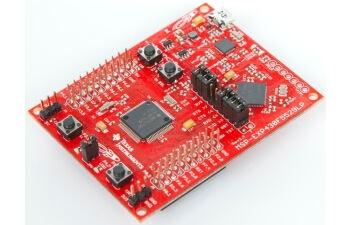
\includegraphics[width=0.7\linewidth]{figuras/launchpad.jpg}
  \caption{LaunchPad Evaluation Kit.}
  \label{fig:launchpad}
\end{figure}

\subsection{BoosterPack}

Os kit de desenvolvimento da disponibilizados pela Texas Instruments têm como foco não só agilizar o desenvolvimento mas também auxiliar na educação, por isso além das LaunchPads a empresa conta com os \textit{BoosterPack plug-in modules}.

Os BoosterPack são módulo que podem ser integrados aos kits de desenvolvimento para fornecer recursos e funcionalidades adicionais para fornecer recursos e funcionalidades adicionais, incluindo recursos de detecção de toque, LCDs e baterias.

